\section{Timers}
In MCUs, we often want a way to periodically do something or
many somethings. Every useful MCU has a hardware timer system.
A \emph{system ticker} (systick) is a special timer reserved for OS
operations, but there is always a timer subsystem outside the CPU
for general use.

The systick timer is a piece of hardware inside the MCU that generates an
systick interrupt signal at fixed intervals. Every interrupt has a dedicated
ISR to handle it, and in the case of systick the ISR is \texttt{SysTick\_Handler}.

In the ARM Cortex-M, the system timer is built into the hardware of the
CPU. Every time an IRQ is raised, the Nested Vectored Interrupt
Controller (NVIC) hardware will determine whether or not to handle the
systick interrupt.

\begin{figure}
    \centering
    \begin{tikzpicture}[node distance=2.2cm and 2.2cm, font=\small]
        \tikzset{
        block/.style   = {draw, thick, rectangle, rounded corners=2pt, minimum width=3.2cm, minimum height=1.2cm, align=center},
        decision/.style= {draw, thick, diamond, aspect=2, inner sep=2pt, align=center},
        line/.style    = {thick, -{Latex[length=3mm]}}
        }

        % Counter and logic
        \node[block] (counter) {Counter\\(24-bit down)};
        \node[decision, right=of counter] (iszero) {count == 0?};
        \node[block, below=1.8cm of iszero] (reload) {Reload original\\value};

        % Connections
        \draw[line] (counter.east) -- (iszero.west);
        \draw[line] (iszero.east) -- ++(1.6,0) node[above, pos=0.45]{No} -- ++(0,1.4) -- ($ (counter.north) + (0,0.8) $) -- (counter.north);
        \draw[line] (iszero.south) -- node[right]{Yes} (reload.north);
        \draw[line] (reload.west) -| (counter.south);

        % Clock waveform feeding the counter
        \coordinate (clkstart) at ($(counter.west)+(-3.2,0)$);
        \node[left] at (clkstart) {Clock};
        \draw[thick]
        (clkstart)
        -- ++(0.6,0) -- ++(0,0.6) -- ++(0.6,0) -- ++(0,-0.6)
        -- ++(0.6,0) -- ++(0,0.6) -- ++(0.6,0);
        \draw[line] ($(clkstart)+(2.4,0)$) -- (counter.west);
    \end{tikzpicture}
    \caption{System Timer}
    \label{fig:systemtimerflowchart}
\end{figure}

When the counter hits zero, \texttt{COUNTFLAG} is set to 1.
The choice of clock input can vary, as most MCUs have multiple.
The clock input is ANDed with a flag to enable and disable.

Let's do an example. Suppose the clock tick frequency $f$ is
80MHz and the goal is a systick
interval $s$ of 10ms. What must the reload value $R$ be?
\begin{align}
    R & = sf - 1                \\
      & = 10ms \times 80MHz - 1 \\
      & = 800000 - 1            \\
      & = 799999
\end{align}

Timers can do far more than just triggering interrupts.
They can also
\begin{itemize}
    \item Capture external events
    \item Drive certain peripherals like GPIO
    \item Output precisely timed signals
\end{itemize}
In output mode, hardware constantly compares the
counter with a value stored in the \emph{compare and capture register}
(CCR), as in figure
\ref{fig:outputmodetimer}.

\begin{figure}
    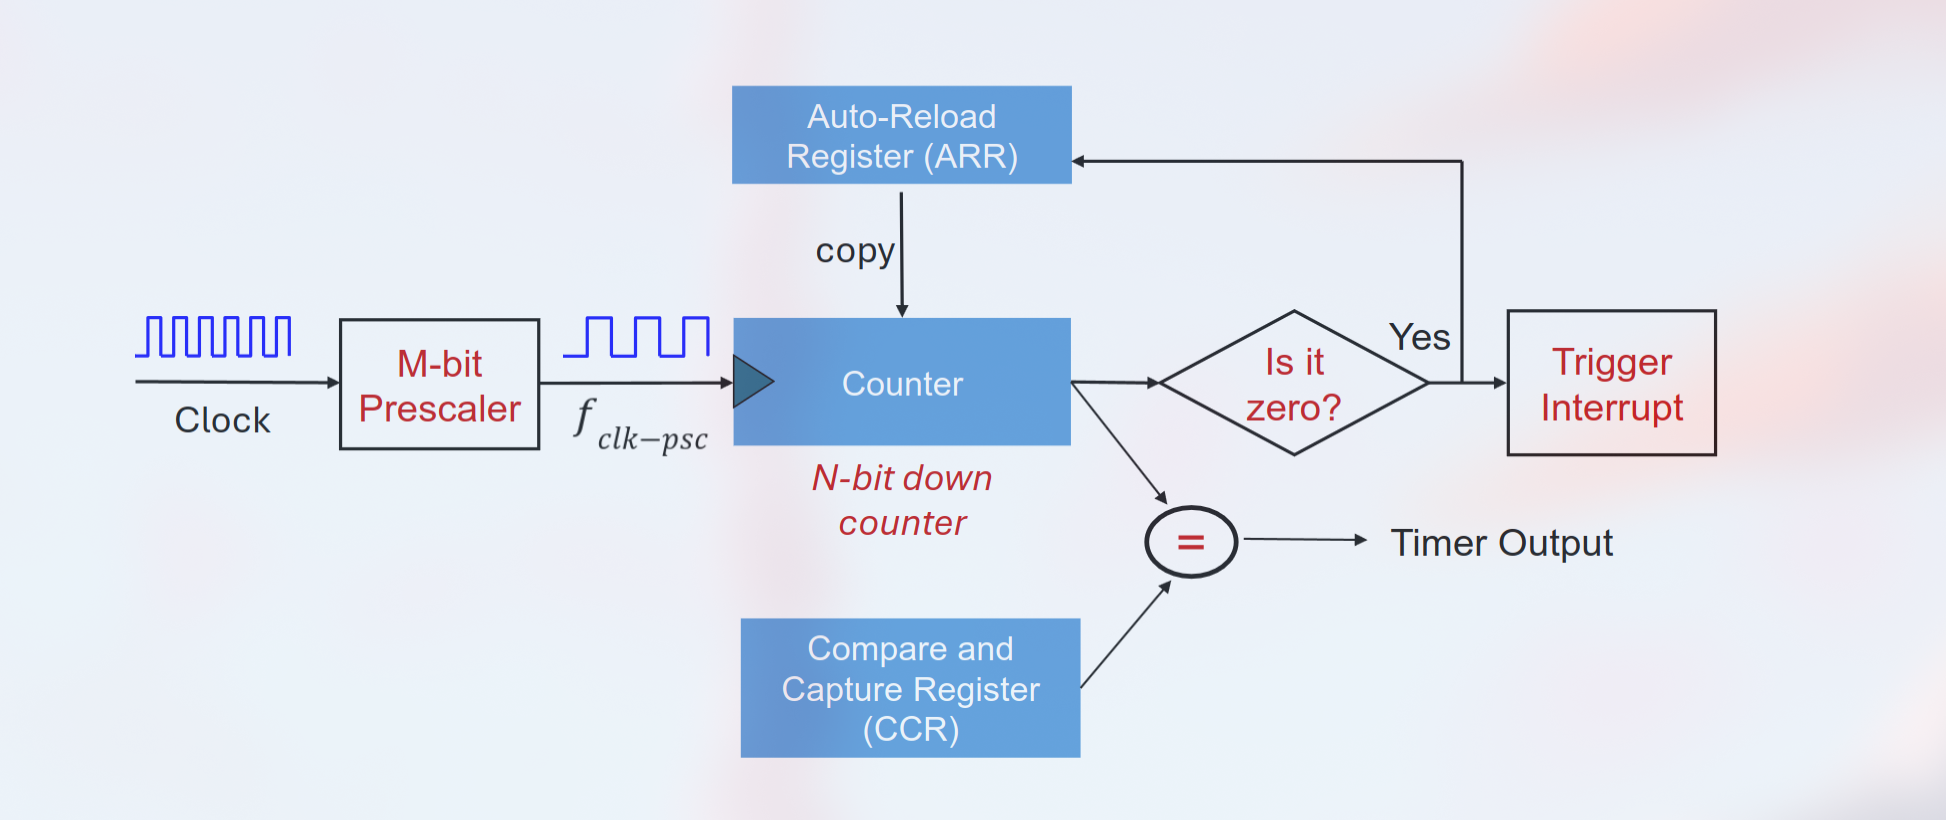
\includegraphics{images/outputmodetimer.png}
    \caption{Timer Output Mode}
    \label{fig:outputmodetimer}
\end{figure}

In general purposes timers, you can count down, up, or up and
down.

The output mode determines what happens when the CCR and counter
are equal. One output mode is active high. When the
timer value equals the CCR, then the timer output is set to high
and stays there. Another output mode is toggle, where the
output switches whenever the timer reaches the CCR value.

\emph{Pulse width modulation} (PWM) is a convenient way to
generate variable duty cycles. You just toggle the output
each time it reaches a given value of the CCR.
\begin{equation}
    \text{Duty Cycle} = \frac{\text{CCR}}{\text{ARR} + 1}
\end{equation}
\begin{equation}
    \text{Period} = (1 + \text{ARR}) \times \text{Clock Period}
\end{equation}
PWM outputs a digital waveform (i.e. either 0 or 1),
with a specific frequency and duty cycle.

We'd like to be able to have a DAC with a strong drive
strength like we have with GPIO.
We don't just want on/off states. We want multiple voltage levels.
Consider a square wave with a varying duty cycle:
We average the area under the curve.
The duty cycle of the wave is then the analog level.
We can average using a low-pass filter.
As long as the wave frequency is much higher than
the signal we want to model, no one will notice
the averaging. We can accomplish averaging with low-pass filters.
Each timer has a PWM mode where the output starts high, and goes low
when CNT == CCRx. The higher the duty cycle, the higher the average.
If the pulse frequency is much higher than that of the
desired signal, the noise will be imperceptible.